\documentclass[11pt]{article}

% some definitions for the title page
\newcommand{\reporttitle}{Popular Network Architectures (\& BatchNorm)}
\newcommand{\reportdescription}{LeNet-5~\cite{LeNet}, MNIST, AlexNet~\cite{AlexNet}, ImageNet, VGG~\cite{VGG}, Inception (GoogleLeNet), BatchNorm~\cite{BatchNorm}, ResNet~\cite{ResNet}, DenseNet, Squeeze-Excite Net U-Net, Data Augmentation}

% load some definitions and default packages
%---------------------------------------------------------------------------
%	PACKAGES AND OTHER DOCUMENT CONFIGURATIONS
%---------------------------------------------------------------------------

\usepackage[twoside]{fancyhdr}
\usepackage{csquotes}

\usepackage[a4paper,hmargin=2.0cm,vmargin=1.0cm,includeheadfoot]{geometry}
% \usepackage{natbib} % for bibliography
\usepackage{biblatex}
\usepackage{tabularx,longtable,multirow,subfigure,caption}%hangcaption
\usepackage{fancyhdr} % page layout
\usepackage{url} % URLs
\usepackage[english]{babel}
\usepackage{graphicx}
\usepackage{rotating}
\usepackage{dsfont}
\usepackage{epstopdf} % automatically replace .eps with .pdf in graphics
% \usepackage{backref} % needed for citations
\usepackage{array}
\usepackage{latexsym}
\usepackage[pdftex,hypertexnames=false,colorlinks]{hyperref} % provide links in pdf (had pagebackref)
\usepackage{booktabs}
\usepackage{wrapfig}
\usepackage{caption}  % Required for \captionof
\usepackage{float} % for H option in figures
\usepackage{amssymb}
\usepackage{amsmath}
\usepackage{amsthm}
\usepackage{mathtools} % for 'dcases*' env.
\usepackage[nottoc]{tocbibind}

%%% Default fonts
\renewcommand*{\rmdefault}{bch}
\renewcommand*{\ttdefault}{cmtt}

%%% Default settings (page layout)
\setlength{\parindent}{0em}  % indentation of paragraph
\setlength{\parskip}{.3em}
\setlength{\itemsep}{0.mm}

\setlength{\headheight}{14.5pt}
\pagestyle{fancy}

\fancyfoot[ER,OL]{\thepage}%Page no. in the left on odd pages and on right on even pages

\fancyfoot[OC,EC]{\sffamily }
\renewcommand{\headrulewidth}{0.1pt}
\renewcommand{\footrulewidth}{0.1pt}
\captionsetup{margin=10pt,font=small,labelfont=bf}

% LISTINGS ammendments
\usepackage{listings}
\usepackage{color}

\definecolor{mygreen}{rgb}{0,0.6,0}
\definecolor{mygray}{rgb}{0.5,0.5,0.5}
\definecolor{mymauve}{rgb}{0.58,0,0.82}

\lstset{ 
  postbreak=\mbox{\textcolor{red}{$\hookrightarrow$}\space},
  backgroundcolor=\color{white},   % choose the background color; you must add \usepackage{color} or \usepackage{xcolor}; should come as last argument
  basicstyle=\footnotesize,        % the size of the fonts that are used for the code
  breakatwhitespace=false,         % sets if automatic breaks should only happen at whitespace
  breaklines=true,                 % sets automatic line breaking
  captionpos=b,                    % sets the caption-position to bottom
  commentstyle=\color{mygreen},    % comment style
%   deletekeywords={...},            % if you want to delete keywords from the given language
%   escapeinside={\%*}{*)},          % if you want to add LaTeX within your code
  extendedchars=true,              % lets you use non-ASCII characters; for 8-bits encodings only, does not work with UTF-8
  firstnumber=1,                % start line enumeration with line 1000
  frame=single,	                   % adds a frame around the code
  keepspaces=true,                 % keeps spaces in text, useful for keeping indentation of code (possibly needs columns=flexible)
  columns=fullflexible,
  keywordstyle=\color{blue},       % keyword style
  language=python,                 % the language of the code
  % morekeywords={*,...},            % if you want to add more keywords to the set
  numbers=left,                    % where to put the line-numbers; possible values are (none, left, right)
  numbersep=5pt,                   % how far the line-numbers are from the code
  numberstyle=\tiny\color{mygray}, % the style that is used for the line-numbers
  rulecolor=\color{black},         % if not set, the frame-color may be changed on line-breaks within not-black text (e.g. comments (green here))
  showspaces=false,                % show spaces everywhere adding particular underscores; it overrides 'showstringspaces'
  showstringspaces=false,          % underline spaces within strings only
  showtabs=false,                  % show tabs within strings adding particular underscores
  stepnumber=1,                    % the step between two line-numbers. If it's 1, each line will be numbered
  stringstyle=\color{mymauve},     % string literal style
  tabsize=2,	                   % sets default tabsize to 2 spaces
  title=\lstname% show the filename of files included with \lstinputlisting; also try caption instead of title
}

% Here, you can define your own macros. Some examples are given below.

\newcommand{\R}[0]{\mathds{R}} % real numbers
\newcommand{\Z}[0]{\mathds{Z}} % integers
\newcommand{\N}[0]{\mathds{N}} % natural numbers
\newcommand{\C}[0]{\mathds{C}} % complex numbers
\renewcommand{\vec}[1]{{\boldsymbol{{#1}}}} % vector
\newcommand{\mat}[1]{{\boldsymbol{{#1}}}} % matrix


\bibliography{bibliography}

\begin{document}

% Include the title page
\begin{titlepage}

    \newcommand{\HRule}{\rule{\linewidth}{0.5mm}} % Defines a new command for the horizontal lines, change thickness here
    
    \center % Center everything on the page
     
    %------------------------------------------------------------------------
    %	HEADING SECTIONS
    %------------------------------------------------------------------------
    
    \textsc{\Large Department of Computing}\\[0.5cm] 
    \textsc{\large Imperial College of Science, Technology and Medicine}\\[0.5cm] 
    
    %------------------------------------------------------------------------
    %	TITLE SECTION
    %------------------------------------------------------------------------
    
    \HRule \\[0.4cm]
    { \huge \bfseries \reporttitle}\\ % Title of your document
    \HRule \\[0.4cm]

    \textit{\reportdescription}
    
    \vspace{2em}

    %------------------------------------------------------------------------
    %	AUTHOR SECTION
    %------------------------------------------------------------------------
    
    \large \emph{Author: Anton Zhitomirskiy}

    \vspace{1em}

    \global\let\newpagegood\newpage
    \global\let\newpage\relax
    
\end{titlepage}

\global\let\newpage\newpagegood

\tableofcontents

\clearpage

\section{LeNet-5}

\begin{figure}[H]
    \centering
    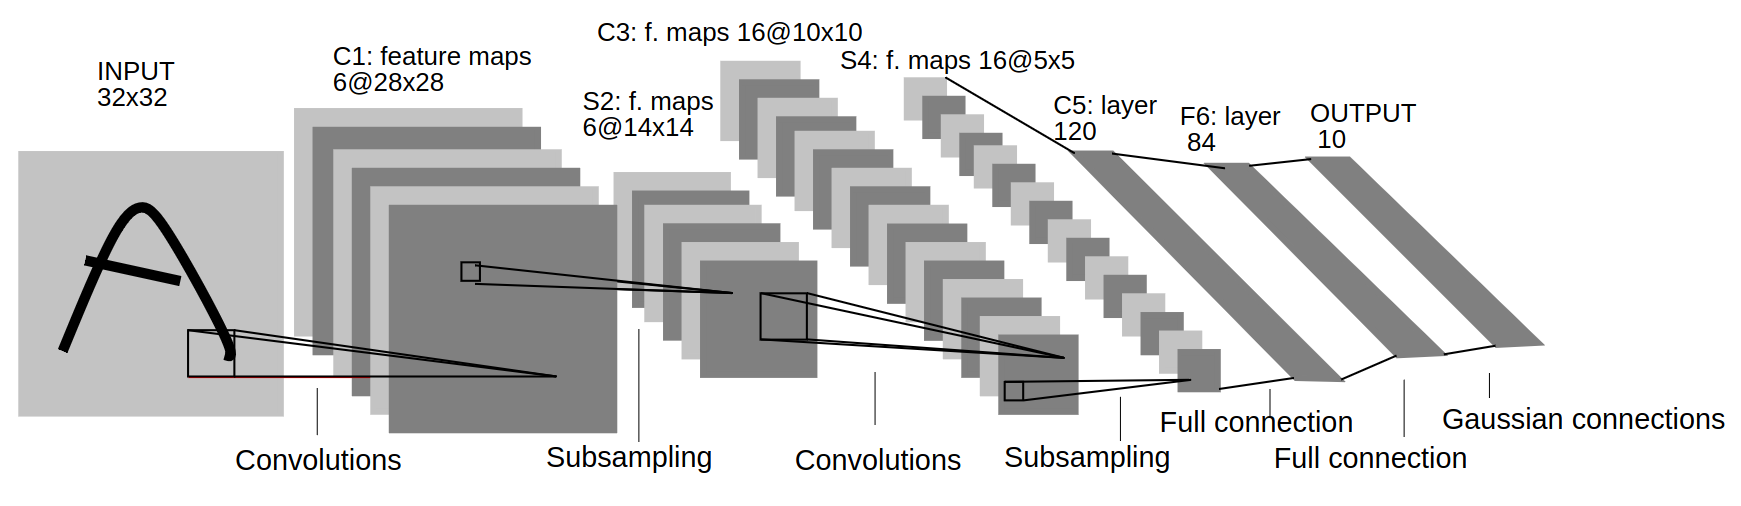
\includegraphics[width=\linewidth]{figures/LeNetFigure.png}
    \caption{Architecture of LeNet-5 a Convolutional Neural Network, here for digits recognition. Each plane is a feature map, i.e. a set of units
    whose weights are constrained to be identical~\cite{LeNet}}
\end{figure}

\lstinputlisting[language=python,firstline=1,lastline=38]{code/LetNet.py}

LeNet~\cite{LeNet} was initially designed for low-resolution, black and white image recognition, specifically for digits. It demonstrated that CNNs could reliably perform both tasks of object localization and recognition (on low-resolution black and white images).

The last steps of the LeNet-5 architecture employ fully connected layers to convert features into final predictions. The scenario of MNIST data didn't matter, because of its small number of output classes. This \textit{complicates the architecture when scaling up, influencing both computational resources and architecture}.

The Convolutional Neural Network Architecture ensures some degree of shift, scale and distortion invariance: \textit{local receptive fields, shared weights} (or weight replication), and spatial or temporal \textit{sub-sampling}.

Once a feature has been detected, its exact location
becomes less important. Only its approximate position
relative to other features is relevant.

\subsection{shared weights}

This algorithm is particularly useful for shared-weight networks because the weight sharing creates ill-conditioning of the error surface. Because of the sharing, one single parameter in the first few layers can have an enormous influence on the output. Consequently, the second derivative of the error with resp ect to this parameter may b e very large, while it can be quite small for other parameters elsewhere in the network

\subsection{sub-sampling}

A simple way to reduce the precision with which the position of distinctive features are encoded in a feature map is to reduce the spatial resolution of the feature map. This can be achieved
with a so-called sub-sampling layers which performs a local
averaging and a sub-sampling, reducing the resolution of
the feature map, and reducing the sensitivity of the output
to shifts and distortions.

\subsection{Loss}

Maximum Likelihood Estimation Criterion (MLE), which is equivalent to the Mean Squared Error (MSE)

\begin{equation*}
    E(W) = \frac 1 P \sum ^ P _{ p = 1} y_{D^P} (Z^P, W)
\end{equation*}

Where $y_{D^P}$ is the output of the $D_p$-th RBF unit, i.e. the one that corresponds to the correct class of the input pattern $Z^p$. 

It lacks three important properties:

\begin{enumerate}
    \item \textbf{Trivial Solution with Adaptation of RBF Parameters}:
        If the parameters of the Radial Basis Function (RBF) are allowed to adapt, the MLE criterion has a trivial and unacceptable solution.
        In this solution, all RBF parameter vectors become equal, leading to a constant and unchanging state of the network.
        The network effectively ignores the input, and all RBF outputs become equal to zero.
    \item \textbf{Lack of Competition Between Classes}:
        The MLE criterion lacks competition between different classes in the training process.
        Introducing a more discriminative training criterion, referred to as the Maximum A Posteriori (MAP) criterion, could address this issue.
        The MAP criterion aims to maximize the posterior probability of the correct class or minimize the logarithm of the probability of the correct class given the input.
        Unlike MLE, MAP introduces a competitive element by pushing up the penalties of incorrect classes in addition to pushing down the penalty of the correct class.
    \item \textbf{Potential Collapsing Phenomenon}:
        When RBF weights are allowed to adapt with the MLE criterion, there is a risk of a collapsing phenomenon where all RBF centers become equal.
        The discriminative criterion of MAP prevents this collapsing effect by keeping the RBF centers apart from each other.
        The discriminative criterion ensures that the posterior probabilities of different classes remain distinct, preventing the network from ignoring the input.
\end{enumerate}

\section{AlexNet}

The AlexNet~\cite{AlexNet} was introduced in 2012 and introduced more layers for larger inputs and larger filters. Originally, the architecture was split into two columns/streams, but this was a workaround for the hardware limitations at the time. 

It used the ImageNet dataset which contained color images with nature objects of larger size compared to MNIST ($469\times 387$ vs $28 \times 28$) and 1.2 million images vs 60k images.

Its key improvements on the LeNet were

\begin{itemize}
    \item Add a dropout layer after two hidden dense layers (better robustness /regularization)
    
    Dropout allowed for much deeper networks by introducing regularization not just at the input layer but throughout multiple layers of the network. This made it possible to control the complexity of the model more effectively.

    \item Change activation function from sigmoid to ReLu (no more vanishing gradient)
    
    enabling training of deeper networks more efficiently.

    \item MaxPooling instead of Average Pooling
    
    This made the learned features more shift-invariant, which is important for object recognition. Max pooling generally retains the most salient features and discards less useful information, making the model more robust.

    \item Heavy data Augmentation like cropping, shifting, and rotation. 
    \item Model ensembling 
    
    Ensemble methods is a machine learning technique that combines several base models in order to produce one optimal predictive model

    \item Using softmax function for classification
    \item Increase in kernel size and stride
    
    design choice to accommodate the higher resolution of images in the ImageNet dataset compared to MNIST.

\end{itemize}

AlexNet is substantially more complex, being about 250 times more computationally expensive. However, it is only ten times larger parametrically than LeNet-5. This way AlexNet is notorious for its high memory usage. 

\begin{figure}[H]
    \centering
    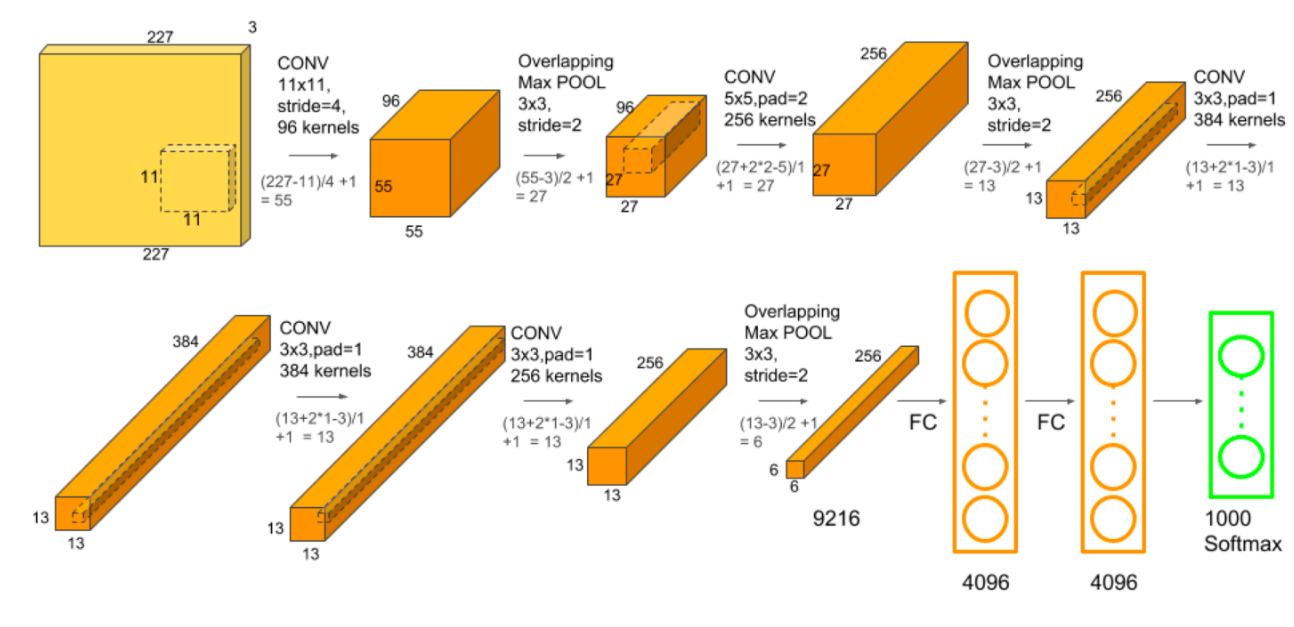
\includegraphics[width=\linewidth]{figures/AlexNetFigure.png}
    \caption{Architecture of AlexNet}
\end{figure}

\lstinputlisting[language=python]{code/AlexNet.py}

\section{VGG}

The Visual Geometry Group~\cite{VGG} uses the `bigger means better' philosophy. VGG introduced the notion of repeated blocks.

\begin{itemize}
    \item \textbf{NOT Add more dense layers} - computationally expensive
    \item \textbf{NOT Add more convolutional layers} - as the network grows, specifying each convolutional layer individually becomes tedious
    \item \textbf{Group Layers into blocks} - these blocks can easily be parameterized, creating a more organized, modular architecture
\end{itemize}

\begin{figure}[H]
    \centering
    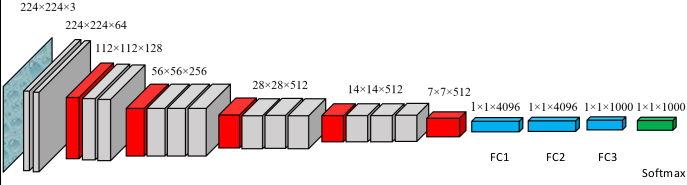
\includegraphics[width=\linewidth]{figures/VGGFigure.png}
    \caption{Architecture of VGG}
\end{figure}

\lstinputlisting[language=python]{code/VGG.py}

\subsection{fewer wide convolutions or more narrow convolutions?}

Recent comprehensive analysis from papers has shown that using more layers of narrow convolutions outperforms using fewer wide ones. This has been a general trend in network design: having more layers of simpler functions is generally more powerful than fewer layers of more complex functions. 

\subsection{The VGG block}

Several $3\times 3$ convolutions, padded by one maintains the spatial dimensions from the input to the output layer, and at the end, max-pooling layer of 2x2 and stride of 2 halves the resolution. 

Combining these blocks with dense layers, creates an entire family of architectures just by varying the number of blocks.

\subsection{Performance}

VGG tends to be a lot slower when compared to the throughput of AlexNet, however, it makes up for in terms of accuracy. While VGG might require more computational resources, it generally provides superior performance.

\begin{warning}
    28.41
\end{warning}

\section{Batch Norm}

The problem deep networks face is with convergence, making training difficult and time consuming. There is a strategy to perform ``deep supervision'' which involves backpropogating from intermediate stages to help the network learn - however, this has its limitations [TODO].

\subsection{Motivation}

Very deep models involve the composition of several functions or layers. The gradient tells how to update each parameter, under the assumption that the other layers do not change. In practice, we update all of the layers simultaneously; gradients flow from the top layer down to the bottom layers of the network. As a result, the last layers start to adapt first, followed by the layers below them, creating a cascade of adaptations throughout the network. 

However, this leads to a problem: As the bottom layers adapt, they change the features that are fed back up to the top layers. This means that the top layers, which had already started to adapt, have to readjust to these new inputs. Training Deep Neural Networks is complicated by the fact that the distribution of each layer's inputs changes during training, as the parameters of the previous layers change~\cite{Goodfellow-et-al-2016}. \textbf{Each layer's learning destabilizes the next, causing a slow convergence process that takes a long time for all layers to adapt properly}.

\subsection{Solution}

Batch normalization can be applied to any input or hidden layer in a network~\cite{Goodfellow-et-al-2016}.

Batch Norm mitigates this issue by normalizing the features within each mini-batch, thereby stabilizing the training process and speeding up convergence. The idea is to make minor corrections to the layers by adjusting their mean and variance during training.

\begin{equation*}
    \mu_B = \frac 1 {|B|}\sum_{i\in B} x_i \quad \sigma^2_B = \frac 1 {|B|} \sum _{i\in B} (x_i - \mu_B)^2 + \epsilon
\end{equation*}

\begin{equation}
    x_{i+1} = \gamma \frac{x_i - \mu_B}{\sigma_B} + \beta\label{eq:batch-norm}
\end{equation}

\begin{center}
Where $\gamma$ is variance and $\beta$ is the mean. $|B|$ represents the size of the mini-batch, and $x_i$ are the individual data points in that mini-batch. $\epsilon$ is a small positive value such as $10^{-8}$ introduced to avoid the potential problem of undefined gradient.
\end{center}

We compute the mean and variance of a given mini-batch during training. Then, re-normalize each input feature by subtracting its mean and dividing it by its standard deviation. The model also learns two parameters to scale ($\gamma$) and shift ($\beta$) the normalized features. 

We then adjust these first and second moments separately from the rest of the network learning, leading to Equation~\ref{eq:batch-norm}. 

\subsection{Advantages}

This way, we are able to ``normalize'' each mini-batch separately, making the training of deep networks more stable and faster (dramatically reducing the number of training epochs required to train deep networks). The normalization can be undone by the network by learning appropriate $\gamma$ and $\beta$ parameters if it sees a benefit to it.

\subsection{Updated Aim}

The original motivation of batch normalization is reducing covariate shift. This is not correct. BatchNorm actually worsens covariate shift, yet it still aids in model convergence. 

\textbf{BatchNorm is effectively acting as a form of regularization by introducing noise into the model}. 

Here's how it works: You calculate the mean and variance of a mini-batch, let's say, of 64 observations. Since you're working with a small sample, both the mean and the variance are subject to noise. You then normalize the features using these noisy statistics, introducing a random scale and shift into your model at each batch. This random noise acts as a regularizing factor, which is why you often don't need additional regularization techniques like dropout when you're using BatchNorm. However, this property makes BatchNorm sensitive to the size of the mini-batch. 

If your mini-batch is too large, you're not introducing enough noise for effective regularization. If it's too small, the noise level becomes counterproductive, affecting convergence. This mini-batch size sensitivity becomes especially significant in multi-GPU settings, where batch sizes are often adjusted.

\subsection{Application}

If you're working with a dense layer, a single normalization is applied to all the activations in that layer.

In the case of a convolutional layer, a separate normalization is performed for each channel.

\subsection{Randomization during use}

You don't want this randomness when you're using the model for predictions. So, you fix the gamma and beta parameters that the model has learned during training. Instead of using batch statistics, you use the running average for the mean and variance to normalize the features.

\printbibliography

\end{document}